\documentclass[english,t]{beamer}
%\documentclass[finnish,english,handout]{beamer}

% Uncomment if want to show notes
% \setbeameroption{show notes}

\mode<presentation>
{
  \usetheme{Warsaw}
  % oder ...
  
  \setbeamercovered{invisible}
  % oder auch nicht
}

% ==============================
%  Added Package
% ==============================
\usepackage[linesnumbered,lined,commentsnumbered]{algorithm2e}
\usepackage{bm}

% =======================================
%   Using symbols for a checklist
% =======================================
\usepackage{pifont}% http://ctan.org/pkg/pifont
\newcommand{\cmark}{\ding{51}}%
\newcommand{\xmark}{\ding{55}}%

% ======================================
%     No Figure in the caption
% ======================================
\setbeamertemplate{caption}{\insertcaption} %---> does not work
%\captionsetup{labelformat=empty,labelsep=none} % ---> it works

% ===================================================
\usepackage{graphicx}
\graphicspath{{./figs/}}
\usepackage[T1]{fontenc}
\usepackage[latin1]{inputenc}
\usepackage{times}
\usepackage{epic,epsfig}
\usepackage{subfigure,float}
\usepackage{amsmath,amsfonts,amssymb}
\usepackage{inputenc}
\usepackage{babel}
\usepackage{afterpage}
\usepackage{eufrak}
\usepackage{amsbsy}
\usepackage{eucal}
\usepackage{rotating}
\usepackage{url}
\urlstyle{same}

\usepackage{natbib}
\bibliographystyle{apalike}

% \definecolor{hutblue}{rgb}{0,0.2549,0.6784}
% \definecolor{midnightblue}{rgb}{0.0977,0.0977,0.4375}
% \definecolor{hutsilver}{rgb}{0.4863,0.4784,0.4784}
% \definecolor{lightgray}{rgb}{0.95,0.95,0.95}
% \definecolor{section}{rgb}{0,0.2549,0.6784}
% \definecolor{list1}{rgb}{0,0.2549,0.6784}
 \definecolor{navyblue}{rgb}{0,0,0.5}
\renewcommand{\emph}[1]{\textcolor{navyblue}{#1}}

% \graphicspath{./pics}

\pdfinfo{            
  /Title      (Bayesian data analysis 2) 
  /Author     (Aki Vehtari) % 
  /Keywords   (Bayesian probability theory, Bayesian inference, Bayesian data analysis)
}


\parindent=0pt
\parskip=8pt
\tolerance=9000
\abovedisplayshortskip=0pt

\setbeamertemplate{navigation symbols}{}
\setbeamertemplate{headline}[default]{}
\setbeamertemplate{headline}[text line]{\insertsection}
\setbeamertemplate{footline}[frame number]


\def\o{{\mathbf o}}
\def\t{{\mathbf \theta}}
\def\w{{\mathbf w}}
\def\x{{\mathbf x}}
\def\y{{\mathbf y}}
\def\z{{\mathbf z}}

\DeclareMathOperator{\E}{E}
\DeclareMathOperator{\Var}{Var}
\DeclareMathOperator{\var}{var}
\DeclareMathOperator{\Sd}{Sd}
\DeclareMathOperator{\sd}{sd}
\DeclareMathOperator{\Gammad}{Gamma}
\DeclareMathOperator{\Invgamma}{Inv-gamma}
\DeclareMathOperator{\Bin}{Bin}
\DeclareMathOperator{\Negbin}{Neg-bin}
\DeclareMathOperator{\Poisson}{Poisson}
\DeclareMathOperator{\Beta}{Beta}
\DeclareMathOperator{\logit}{logit}
\DeclareMathOperator{\N}{N}
\DeclareMathOperator{\U}{U}
\DeclareMathOperator{\BF}{BF}
\DeclareMathOperator{\Invchi2}{Inv-\chi^2}
% \DeclareMathOperator{\Pr}{Pr}
\def\euro{{\footnotesize \EUR\, }}
\DeclareMathOperator{\rep}{\mathrm{rep}}


% ============
% Otsikko sivu
% ============

\title[]{Dasar Pemrograman part I}
\subtitle{}

\author{Hendra Bunyamin}

\institute[  Maranatha]
{
	\normalsize
	\hfill \break
	\hfill \break
  \textbf{Program Studi Teknik Informatika} \\
  \textbf{Fakultas Teknologi \& Rekayasa Cerdas} \\
  \textbf{Universitas Kristen Maranatha} 
  
  \bigskip 
  \textit{13 Agustus 2025}
}


\date[NUNI IT Online] % (optional, should be abbreviation of conference name)
{
%	\begin{center}
\noindent 
\includegraphics[scale=.05]{images/logo-ftrc+text-abu} 
%	\end{center}
		
%	\newline \newline 26 Mei 2021 \\ \bigskip  \bigskip  \bigskip \bigskip 
\includegraphics[scale=.05]{images/logo-ftrc+text-abu}
}



%\pgfdeclareimage[height=1.5cm]{university-logo}{images/logo-mcu}
%\logo{\pgfuseimage{university-logo}}
\AtBeginSection[]
{
  \begin{frame}<beamer>{Outline}
    \tableofcontents[currentsection,currentsection]
  \end{frame}
}


\begin{document} 

\begin{frame}
  \titlepage
\end{frame}

\begin{frame}{Outline}
  \tableofcontents
  % You might wish to add the option [pausesections]
\end{frame}

\section{Tulis Statement C++}
\begin{frame}{Tulis Statement C++ \citep{deitel2003c++}}
\begin{enumerate}
	\item  Print the message \texttt{"Enter two numbers"}.
	\item Assign the product of variables \texttt{b} and \texttt{c} to variable \texttt{a}.
	\item Input three integer values from the keyboard into integer variables \texttt{a}, \texttt{b}, and \texttt{c}.
\end{enumerate}
\end{frame}

%%%%
\section{Statement untuk Equation}
\begin{frame}{Statement untuk Equation}
	Given the algebraic equation $y=ax^3 + 7$, which of the following, if any, are correct C++ statements for this equation?
	\begin{itemize}
		\item[A.] \texttt{y = a * x * x * x + 7;}
		\item[B.] \texttt{y = a * x * x * (x + 7);}
		\item[C.] \texttt{y = (a * x) * x * (x + 7);}
		\item[D.] \texttt{y = (a * x) * x * x + 7;}
		\item[E.] \texttt{y = a * (x * x * x) + 7;}
		\item[F.] \texttt{y = a * x * (x * x + 7);}
	\end{itemize}
\end{frame}

\section{Arithmetic}
\begin{frame}{Arithmetic}
Write a program that asks the user to enter two numbers, obtains the two numbers from the user and prints the sum, product, difference, and quotient of the two numbers.	
\end{frame}

\section{Arithmetic, Smallest, and Largest}
\begin{frame}{Arithmetic, Smallest, and Largest}
Write a program that inputs three integers from the keyboard and prints the sum, average, product, smallest and largest of these numbers. The screen dialog should appear as follows:
\begin{center}
	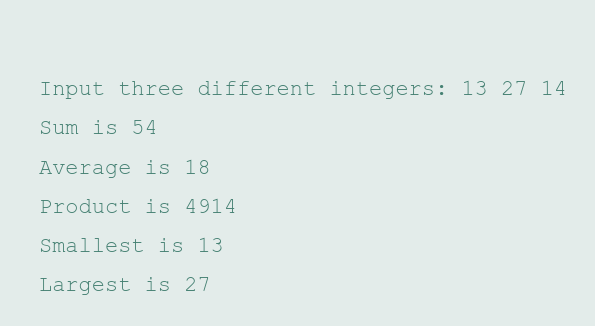
\includegraphics[scale=.5]{images/arithmetic+largest+smallest}
\end{center}
\end{frame}

\section{Diameter, Circumference and Area of a Circle}
\begin{frame}{Diameter, Circumference and Area of a Circle}
	Write a program that reads in the radius of a circle as an integer and prints the circle?s diameter, circumference and area. Use the constant value 3.14159 for ?. Do all calculations in output statements. 
\end{frame}

\section{Odd or Even}
\begin{frame}{Odd or Even}
	Write a program that reads an integer and determines and prints whether it's odd or even. \\
	$[$Hint: Use the remainder operator (\%). An even number is a multiple of two. Any multiple of 2 leaves a remainder of zero when divided by 2.$]$
\end{frame}

\section{Digits of an Integer}
\begin{frame}{Digits of an Integer}
	Write a program that inputs a five-digit integer, separates the integer into its digits and prints them separated by three spaces each. [Hint: Use the integer division and remainder operators.] For example, if the user types in \texttt{42339}, the program should print:
\begin{center}
	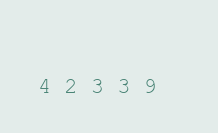
\includegraphics[scale=.5]{images/digits-integer}
\end{center}
\end{frame}

%
%\begin{frame}{Hello World!}
%\begin{algorithm}[H]
%	\SetKwData{Left}{left}
%	\SetKwData{This}{this}
%	\SetKwData{Up}{up}
%	\SetKwFunction{Union}{Union}
%	\SetKwFunction{FindCompress}{FindCompress}
%	\SetKwInOut{Input}{Input}
%	\SetKwInOut{Output}{Output}
%
%\Input{Suatu bil$Im$ of size $w\times l$ \\ and $n$}
%\Output{A partition of the bitmap}
%\BlankLine   
%\emph{special treatment of the first line}\;
%\For{$i\leftarrow 2$ \KwTo $l$}{
%	\emph{special treatment of the first element of line $i$}\;
%	\For{$j\leftarrow 2$ \KwTo $w$}{\label{forins}
%	\Left$\leftarrow$ \FindCompress{$Im[i,j-1]$}\;
%	\Up$\leftarrow$ \FindCompress{$Im[i-1,]$}\;
%	\This$\leftarrow$ \FindCompress{$Im[i,j]$}\;            
%	\If(\tcp*[h]{O(\Left,\This)==1}){\Left compatible with \This}{\label{lt}
%		\lIf{\Left $<$ \This}{\Union{\Left,\This}}
%		\lElse{\Union{\This,\Left}}
%	}
%	\If(\tcp*[f]{O(\Up,\This)==1}){\Up compatible with \This}{\label{ut}
%		\lIf{\Up $<$ \This}{\Union{\Up,\This}}
%		\tcp{\This is put under \Up to keep tree as flat as possible}\label{cmt}
%		\lElse{\Union{\This,\Up}}\tcp*[h]{\This linked to \Up}\label{lelse}
%		}
%	}   
%	\lForEach{element $e$ of the line $i$}{\FindCompress{p}}
%	}
%	\caption{disjoint decomposition}\label{algo_disjdecomp} 
%\end{algorithm}
%\end{frame}









%%%% predictive distribution


 % \begin{frame}
 %   \frametitle{Some other one parameter models}

 %   \begin{itemize}
 %   \item Poisson
 %   \item Exponential
 %   \item Cauchy
 %   \end{itemize}
   
 % \end{frame}

\section<presentation>*{\appendixname}
\subsection<presentation>*{For Further Reading}

\begin{frame}[allowframebreaks]
  \frametitle<presentation>{Daftar Pustaka}
    {\footnotesize
%    \bibliographystyle{apalike}
    \bibliography{references}
    }    
\end{frame}

\end{document}

%%% Local Variables: 
%%% TeX-PDF-mode: t
%%% TeX-master: t
%%% End: 
